\documentclass[12pt,a4paper]{article}
\usepackage[left=25mm,right=15mm,top=15mm,bottom=15mm]{geometry}
\usepackage[utf8x]{inputenc}
\usepackage[L7x]{fontenc}
\usepackage[lithuanian]{babel}
\usepackage{url}
\usepackage{float}
\usepackage{graphicx}
\renewcommand{\baselinestretch}{1.2}
\graphicspath{ {img/} }

\begin{document}
\begin{titlepage}
  
  \begin{center}
    \textsc{\LARGE Vilniaus Gedimino Technikos universitetas}\\[2mm]
    \textsc{\Large Elektroninių sistemų katedra}\\[70mm]
    \textsc{\Large Automatizuotas žinių išgavimas, sistemos}\\[10mm]
    \textsc{\normalsize Žinių inžinerijos referatas}\\[40mm]
    \begin{minipage}{1\textwidth}
      \begin{flushright}
        \emph{Darbą atliko:} Maksim Norkin, AKSfm-15\\
        \emph{Darbą tikrino:} Juozas Laučius\\
      \end{flushright}
    \end{minipage}
    \vfill
    {\large Vilnius \\ \the\year}
  \end{center}
\end{titlepage}
\tableofcontents
\newpage

\section{Įvadas}

Objekto padėties nustatymas turi dvi plačias pritaikymo sritis: inercinė navigacinė ir žmogaus judesio sekimo sistema \cite{schlomer2008gesture};

Objekto pozicijos nustatymas, panaudojus inercinius jutiklius remiasi prielaida, jog objektas lieka ramybės būsenoje tol, kol jį nepaveikia išorinė jėga. Tokia jėga suteikia objektui pagreitį. Jeigu rasta pagreitį galima išmatuoti ir suintegruoti, pagreičio ir pozicijos kitimas gali būti išmatuoti. Reikia nepamiršti, kad tokiu atveju matavimą sudarys dvi komponentės -- pagreitis dėl gravitacijos ir išorinės veikiančios jėgos pagreitis. Norint pašalinti gravitacijos komponentę iš pagreičio matavimo, reikia žinoti kokiu kampu akcelerometras yra vertikalės atžvilgiu.
Tokio kampo matavimui, reikalingas kitas jutiklis, kuris vadinasi giroskopas. Jis matuoja kampo greitį, kurį matematiškai integruojant, galima rasti kampo greičio pokytį nuo pradinio, žinomo kampo \cite{sukkarieh2000low}.

Akcelerometras suteikia pagreičio matavimą norimam objektui. Dažniausiai tokie matavimai yra užrašomi $x$, judėjimą tiesiai, $y$, šonu ir $z$ vertikaliai. Giroskopas suteikia matavimus, kurie dengia nurodytas ašis ir yra užrašomi $\theta$, sūkiui, $\beta$ polinkiui ir $\gamma$ vingiavimui, kaip pavaizduota \ref{tikz:axis_of_the_system} pavyzdyje. Tokių inercinių įverčių naudojimas turi pagrindinį privalumą -- stebimo objekto polinkis ir pagreitis gali būti vertinami bet kokioje navigacijoje.  

\begin{figure}[H]
    \centering
    \caption{Objekto pozicijos pagreičio pokyčio ašys, $x$, $y$ ir $z$. Sūkio matmenys apie ašis $\theta$, $\beta$ ir $\gamma$.}
    \label{tikz:axis_of_the_system}
    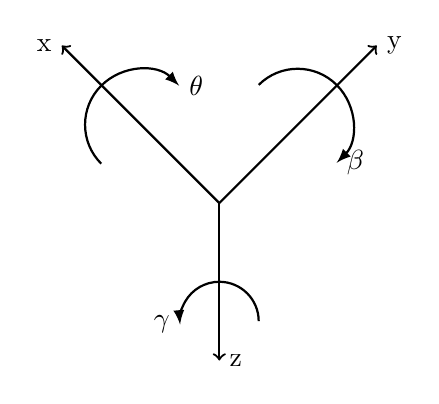
\begin{tikzpicture}
        % axis
        \draw[thick, black, ->] (0,0) -- ( 2, 2) node [right] {y};
        \draw[thick, black, ->] (0,0) -- (-2, 2) node [left] {x}; 
        \draw[thick, black, ->] (0,0) -- ( 0,-2) node [right] {z};
        % arc
        \draw[thick, -latex] ( 0.5,  1.5) arc (135:-45:0.70) node [right] {$\beta$}; 
        \draw[thick, -latex] (-1.5,  0.5) arc (225:45:0.70) node [right] {$\theta$};
        \draw[thick, -latex] ( 0.5, -1.5) arc (0:185:0.5) node [left] {$\gamma$};
    \end{tikzpicture}
\end{figure}

Inercinės navigacijos sistemos yra naudojamos labai plačiai lėktuvuose, raketose, kosmoso laivuose, povandeniniuose ir vandens laivuose \cite{woodman2007introduction}. Progresas gaminant MEMS įrenginius, sudarė galimybes kurti mažas ir lengvas navigacines sistemas. Tokie privalumai leidžia praplatinti įrenginių panaudojimo galimybes ir šiuo metu įtraukia tokias sritis kaip žmogaus ir gyvūnų judesio sekimą.

Tačiau reikia nepamiršti ir apie klaidas, kurias sukelia nuolatinė dedamoji, santykio įverčiai ir nelinijines sistemos įtakos jutiklio verčių nuskaitymo metu. Tokios klaidos yra pagrindinė priežastis atsirasti netikslumams navigacinėje sistemoje per laiko vienetą. Netikslumai sąlygoja akselerometro įverčius, kuriuos tampa labai sunku atskirti tarp gravitacinio lauko ir objekto judėjimo, ko pasekoje objekto pozicijos matavimas toliau yra dar netikslesnis. Kadangi inerciniai jutikliai yra tokio tipo, kuriems yra labai svarbi tiksli prieš tai buvusi pozicija, bet kokia klaida skaičiuojant prieš tai buvusia pozicija, įtakoja ir dabartinės pozicijos skaičiavimą. Tokiu būdu, su laiku navigacinė sistema tampa visiškai netiksli ir praranda visą savo vertę.

\section{Istorija}

Duomenų gavybos ištakas galima paaiškinti kaip natūralią informacinių technologijų evoliuciją. 
Duomenų bazės ir duomenų valdymo industrija evoliucionavo iš poros kritinių funkcionalumų vystymo: duomenų surinkimas ir duomenų bazės sukūrimas, duomenų valdymas ir pažangus duomenų analizavimas. 
Ankstyvi duomenų surinkimo ir duomenų bazių kūrimo mechanizmai veikę kaip pagrindas tolimesniam efektyvesnių mechanizmų vystymui duomenų skaitymui ir rašymui, kaip ir užklausos ir transakcijos apdorojimui.
Dabartinės duomenų bazių sistemos jau numatytai suteikia užklausos ir transakcijos apdorojimą.
Pažangus duomenų analizavimas natūraliai tampa sekančiu žingsniu. 

Nuo 1960 metų, duomenų bazės ir informacinės technologijos evoliucionavo sistematiškai nuo primityvių bylų apdorojimo sistemų iki rafinuotos ir galingos duomenų bazės sistemos.
Tyrimas ir duomenų bazių įgyvendinimas nuo 1970 metų pažengė nuo hierarchinių ir tinklo duomenų bazių sistemų iki reliacinės sistemos, duomenų modeliavimo įrankių, indeksavimo ir priėjimo metodų.
Taip pat, naudotojai gavo labai praktinį ir lankstų priėjimą prie duomenų per užklausos kalbas, naudotojo sąsajas, užklausos optimizavimą ir transakcijos valdymą.
Efektyvūs metodai tinklo transakcijos apdorojimui, kur į užklausą yra žvelgiama kaip į skaitymo transakcija, suvaidino svarbų vaidmenį plačioje reliacinės technologijos adaptacijoje, kaip pagrindinį įrankį efektyviam duomenų saugojime, skaityme ir didelių duomenų kiekio valdyme.

Pažangios duomenų analizės sistemų vystymas prasidėjo nuo  1980 metų.
Stabilus ir neįtikėtinas kompiuterinės įrangos progresas per ankstesnius tris dešimtmečius suteikė pažangių ir pigių kompiuterių -- duomenų surinkimo, saugojimo įrenginių.
Tokia technologija leido labai pasitempti duomenų bazių ir informacinių technologijų industrijai. Ji leido didelius kiekius duomenų bazių ir informacijos saugyklų būti pasiekiamai per transakcija, informacijos nuskaitymą, bei duomenų analizę.
Dabar duomenys gali būti saugojami skirtingose duomenų bazių saugyklose.

Viena sparčiausiai augančių duomenų saugojimo architektūrų yra \textit{data warehouse}.
Tai yra didelė struktūra iš kelių skirtingų duomenų šaltinių, organizuotų po viena duomenų schema vienoje vietoje, kuri įgalina priiminėti sprendimus.
Duomenų centro technologija susideda iš duomenų valymo, duomenų integravimo ir analitinio tinklo apdorojimo -- analizavimo technikos, iš išvadų sudarymo, įtvirtinimo ir agregavimo. Taip pat galimybė peržiūrėti informaciją iš skirtingų kampų.
Nors šie įrankiai leidžia daugybės dimensijų analizavimą ir priimti kažkokį sprendimą, papildomi analizės įrankiai yra reikalingi gilesnei analizei, kaip pavyzdžiui duomenų gavybos įrankiai, kurie suteikia galimybe klasifikavimui, grupavimui, neįprastiems požymiams rasti ir pokyčių ieškojimui per laiko tarpą.

Dideli kiekiai duomenų taip pat yra surenkami už duomenų bazių ir saugojimo stočių. Per 1990 atsirado bendras interneto tinklas ir su juo pradėjo labai sparčiai plisti internetinės duomenų bazės, kaip pavyzdžiui yra \textit{XML}.
Tinklu paremtos informacijos bazės iškilo ir turi labai svarbią sritį informacinėje srityje.
Efektyvi ir naudinga tokių duomenų formos analizė yra labai didelis ir sunkus uždavinys.

Susidaro labai didelė problema -- didelis skaičius duomenų nesąlygoja visiškai kažkokių žinių, kurias suteikia toks jų skaičius.
Limitas, kuris nusako vieno žmogaus sugebėjimus analizuoti duomenis ir išgauti iš jų kažkokia informacija rankiniu būdu jau seniai yra peržengta.
Tokiu būdu duomenų saugyklos tapo tiesiog duomenų kapinėmis, kurias niekas neanalizuoja.
Tokiu būdu kritiniai sprendimai yra dažniausiai priimami ne atsižvelgiant į informaciją, kuri gali būti išgauta iš turimų surinktų duomenų, o į priimančios pusės intuicijos.
Buvo atlikti bandymai rankiniu būdu integruoti duomenys ir srities žinias priiminėti tam tikrus sprendimus, tačiau toks bandymas nepavyko, kadangi tokios sistemos dažniausiai yra stipriai veikiamos žmonių nešališkumo.
Labai reikia sistemiškai atlikinėti žinių išgavimo įrankių vystymą, tuomet esami duomenų kapai taps auksiniais kiaušiniais.





\section{Kas yra žinių išgavimas}

Žinių išgavimas gali būti apibūdinamas labai skirtingai, kadangi šitas mokslas priklauso daugeliui sričių.
Netgi terminas \textit{žinių išgavimas}, nesudaro viso bendro vaizdo.
Terminas turėtų būti labiau susijęs su sritimi, kaip pavyzdžiui ``žinių išgavimas iš duomenų'', tačiau jis yra labai ilgas.

Daugelis žmonių žinių išgavimą laiko sinonimu su ``žinių atradimui iš duomenų'', tuo tarpu kiti į terminą žiūri tiesiog kaip svarbų žingsnį žinių atradimo procese. Žinių atradimo procesas susideda iš žingsnių:

\begin{itemize}
    \item Duomenų valymas. Triukšmo ir netolydžių duomenų šalinimas.
    \item Duomenų integravimas. Jeigu yra keli duomenų šaltiniai ir juos reikia sujungti.
    \item Duomenų pasirinkimas. Duomenys, kurie turi svarbą nagrinėjamam atvejui yra nuskaitomi iš duomenų bazės.
    \item Duomenų transformavimas. Duomenys yra transformuojami ir sudaromi į formas, kurios yra tinkamos išgavimui, ir yra galimos bendrinimo ir grupavimo operacijos.
    \item Duomenų išgavimas. Svarbus žingsnis, kuriuo metu yra pritaikomi intelektualūs įrankiai išskirti modeliui.
    \item Modelio įvertinimas. 
    \item Žinių pateikimas. Vizualus rasto modelio pateikimas naudotojui.
\end{itemize}

Nurodyti žingsniai parodo, kad žinių išgavimas yra žinių atradimo proceso dalis, tiksliau galima pasakyti, kad šitas žingsnis yra esminis, kadangi jis atskleidžia paslėptus modelius, kuriuos galima vertinti.
Reikia pastebėti, jog industrijoje, žiniasklaidoje ir tyrimuose, žinių išgavimo sąvoka naudojama išreikšti visą žinių atradimo procesą, dėl trumpumo.
Dėl šios priežasties, žinių išgavimo funkcionalumas yra apibūdinamas kaip įdomių modelių ir žinių atradimas iš didelio skaičiaus duomenų.
Duomenų šaltinis gali būti duomenų bazės, saugyklos, internetas ir kitos informacijos talpyklos, arba duomenys, kurie yra gaunami srautu, dinamiškai.

\section{Kokias žinias galime išgauti}

Kaip taikoma technologija, žinių išgavimas gali būti taikomas bet kokio tipo duomenims, kol tai yra naudojama kažkokiam konkrečiam tikslui su savo uždaviniu.
Pačios paprasčiausios žinių išgavimo formos yra programos, kurios yra orientuotos į duomenų, duomenų saugyklos ir perdavimo duomenis.
Šioje apžvalgoje aptarsime būtent tokias programas.

\subsection{Duomenų bazės}

Duomenų bazės sistema, anglų kalboje sutrumpintai taip pat vadinama \textit{DBMS}, susideda iš viduje sujungtų duomenų rinkinio, kitaip vadinami baze, yra rinkinys programų, kurios yra skirtos dirbti su duomenimis.
Programinis paketas suteikia galimybes nusakyti duomenų struktūras ir duomenų saugojimą. Kitas kritinis aspektas, kurį sprendžia programinis paketas yra tuo pačiu metu vykdomą, paskirstytą duomenų manipuliavimą bei duomenų integracijos palaikymą, saugumą, nepriklausomai ar sistema buvo prieš tai išjungta ar buvo įvykęs neleistinas priėjimas prie duomenų.

Sąryšinė duomenų bazė yra lentelių rinkinys, kurio kiekviena turi savo unikalų vardą. Kiekviena lentelė susideda iš atributų rinkinio (stulpelių pavadinimas), ir dažniausiai joje yra saugomas didelis duomenų skaičius (eilutės). 
Kiekviena eilutė sąryšinėje lentelėje pavaizduoja objektą, kuris yra atpažįstamas pagal unikalų raktą, aprašytą objekto atributų rinkinio. 
Semantinis duomenų modelis, dar žinimas kaip esybės sąryšio duomenų modelis, yra dažniausia konstruojamas per sąryšinę duomenų bazę.
Semantinis duomenų modelis vaizduoja duomenų bazę kaip esybių ir jų sąryšių santykius.

Sąryšinė duomenų bazė gali būti prieinama per duomenų bazės užklausas, kurios yra parašytos sąryšine kalba, angliškai vaidinama \textit{SQL} arba per palaikoma kalbos grafinę aplinką. 
Duota užklausa yra transformuojama į sąryšines operacijas, kaip pavyzdžiui \textit{join}, \textit{select} ir \textit{project} ir tuomet yra optimizuojama efektyviam apdorojimui.
Užklausa leidžia gauti specifinį duomenų poaibį.
Galima įsivaizduoti tokią situacija, kuomet reikia išanalizuoti \textit{AllElectronics} duomenis. 
Naudojant sąryšio užklausas, galima pateikti tokias užklausas kaip ``Parodyk man sąrašą elementų, kurie buvo parduoti paskutiniam ketvirtyje''. 
Sąryšio kalbos taip pat pateikia kai kuriuos duomenų grupavimo įrankius, kaip sumavimas, vidurkis, skaičiavimas, maksimumas ir minimumas.
Grupavimo operacijos leidžia užklausti tokių klausimų kaip: ``Parodyk man visus pardavimus už praeitą mėnesį, grupuojant pagal atstovybę'' arba ``Kiek įvyko sandorių per Gruodį?'' arba ``Koks pardavimo vadybininkas turėjo daugiausiai pardavimų?''.

Kuomet yra vykdomas žinių išgavimas iš sąryšinės duomenų bazės, galima judėti toliau ir ieškoti duomenų tendencijų ir duomenų modelių.
Pavyzdžiui, žinių išgavimo sistemos gali analizuoti klientų duomenis ir nustatyti naujų klientų kredito rizikos grupę, sprendžiant pagal jų pajamas, amžiaus grupę ir buvusią kredito informaciją.
Duomenų analizavimo sistemos taip pat gali įvertinti duomenų nuokrypius -- pavyzdžiui galima pagauti tokius pardavimus, kurie buvo netikėti, lyginant su praeitu laikotarpiu.
Tokie nuokrypiai gali būti toliau išnagrinėti.
Pavyzdžiui, žinių išgavimo metodas gali nustatyti, kad tuo metu buvo atliktas pakavimo medžiagos pakeitimas, arba mažas kainos padidėjimas.

Sąryšinės duomenų bazės yra daugiausiai pasiekiamos ir turtingiausios duomenimis saugyklos. 
Kas sąlygoja labai platų jų naudojimą žinių išgavimo sistemose.

\subsection{Duomenų saugyklos}

Įsivaizduokime, jog \textit{AllElectronics} yra sėkminga tarptautinė įmonė, su savo atstovybėmis aplink pasaulį.
Kiekviena atstovybė turi savo sąrašą duomenų bazių.
Įmonės direktorius paprašė analitinės informacijos apie įmonės pardavimus per vieną kiekvieno įrenginio tipo vienetą kiekviename iš atstovybės šiame trečiame ketvirtyje.
Tai yra sudėtingas uždavinys, kadangi reikiami duomenys yra paskirstyti per skirtingas duomenų bazes, kurios yra fiziškai skirtingose vietose.

Tokia problema sprendžia duomenų saugyklos.
Saugykla yra informacijos sandėlis, kuris yra surenkamas iš daugelio šaltinių, patalpinamas bendroje schemoje, ir gyvena vienoje vietoje.
Saugyklos yra konstruojamos per procesą, kuris susideda iš duomenų valymo, integravimo, transformavimo, įkrovimo ir periodinio duomenų atnaujinimo.

Sprendimo priėmimo palengvinimui, duomenys saugykloje yra organizuojami pagal tam tikras sritis -- klientas, įrankis, tiekėjas ar įvykis.
Duomenis, kurie teikia kažkokius istorinius duomenis per kažkokį laikotarpį -- pavyzdžiui 6, 12 mėnesio laikotarpiui, dažniausiai yra apibendrinama.
Pavyzdžiui vietoje to, kad saugoti detalią informaciją apie kiekvieną iš atliktų pardavimų, duomenų saugykla gali saugoti tik išvadas apie visas transakcijas pagal objektą kiekvienai parduotuvei ar dar aukštesniu lygiu -- per kiekvieną iš pardavimo regionų.

Duomenų saugyklos dažniausiai modeliuojamos aukštų dimensijų duomenų struktūros, dar vadinamos duomenų kubais, kuriame kiekviena dimensija atitinka atributui ar atributų rinkiniui schemoje, ir kiekviena ląstelė saugo grupuoto įverčio reikšmę, kaip skaičių ar sumą. Duomenų kubas suteikia daugelio dimensijų vaizdą į duomenis ir juos parengia greitam priėjimui.

Pateikiant daugelio dimensijų vaizdą į duomens ir atliekant pasiruošimą skaičiavimams su grupuotais duomenimis, duomenų saugyklos leidžia paveldėti realaus laiko analizavimo procesą. 
Jis leidžia atlikti operacijas pasinaudojant esamomis žiniomis apie dalyką, kurio duomenys yra analizuojami, ir tai leidžia pateikti duomenis skirtingose abstrakcijos lygiuose.
Tokios operacijos surenka skirtingus naudotojų vaizdo taškus.
Realaus laiko analizavimo proceso pavyzdys gali būti kasimasis žemyn, ar surišimas, kurie yra atliekami naudotojo peržiūrint duomenis skirtingais grupavimo kampais.
Pavyzdžiui kasimasis žemyn operacija gali būti pritaikyta pardavimų duomenims kiekvienam ketvirčiui, norint pamatyti duomenis kiekvienam mėnesiui.
Panašiu principu galima surišti duomenis kiekvienam miestui, ir peržvelgti grupuotą informaciją pagal šalį.

Nors duomenų saugyklų įrankiai padeda atlikti duomenų analizavimą, tačiau yra reikalingi ir papildomi duomenų analizės įrankiai.
Daugelio dimensijų žinių išgavimas (taip pat žinomas kaip žvalgomasis daugelio dimensijų žinių išgavimas) atliekamas žinių išgavimo daugelio dimensijų realaus laiko analizavimo plokštumos stiliuje.
Tai reiškia, kad yra atliekama žvalgyba kaip priklauso skirtingos grupuotų duomenų dimensijos per skirtingus ryškumo lygius, kas labai padidina galimybes surasti įdomius duomenų modelius, kurie gali pateikti labai įdomią informaciją apie nagrinėjamą sritį.

\subsection{Transakcijos duomenis}

Apskritai, kiekvienas įrašas sandorio duomenų bazėje įrašo transakciją -- pirkėjo pirkinys, skrydžio rezervacija, naudotojo mygtuko paspaudimas tinklalapyje.
Transakcija dažniausiai sudaro identifikuojamas unikalus transakcijos numeris ir sąrašas duomenų, kurie įtvirtina transakciją.
Duomenų bazė gali turėti papildomas lenteles, kurios susideda iš kitos informacijos, susiejama su transakcija, kaip pavyzdžiui daikto aprašymas, informacija apie pardavėja arba atstovybę.

Analitikas \textit{AllElectronics} gali paklausti ``Kokie įrenginiai buvo parduoti kartu?''.
Tokia pirkinių krepšelio duomenų analizė leistų sujungti grupę įrenginių kartu ir leistu padidinti pardavimų skaičių.
Pavyzdžiui, žinant, kad spausdintuvai yra dažniausiai perkami kartu su kompiuteriais, galima pateikti pasiūlymą pirkėjams įsigyti spausdintuvą už labai žemą kainą arba netgi už dyką visiems pirkėjams, kurie perka pasirinktus kompiuterius. Taip tikėtis, jog bus parduota daugiau kompiuterių.
Standartinė duomenų bazė nesugeba atlikti pirkinių krepšelio tipo analitinės operacijos.
Sandorio tipo duomenų bazėse galima atlikti sandorio dažniausią sąrašą objektų grupių -- rasti objektus, kurie buvo dažnai nupirkti kartu.

\subsection{Kiti duomenis}

Neskaitant sąryšio duomenų bazių, saugyklų, sandorio bazių, egzistuoja daug kitų skirtingų duomenų saugyklų, kurios turi skirtingas formas ir struktūras ir semantines reikšmes.
Tokie duomenis gali būti matomi daugelio taikymo srityse -- laiko ar įrašo eilės duomenys (istoriniai duomenis, biržos pardavimo duomenis, biologinės eilės duomenis), duomenų srautai (vaizdo stebėjimas ir jutiklių duomenis, kurie yra perduodami nuolatos), erdviniai duomenis (žemėlapiai), inžineriniai projektavimo duomenys (pastatų projektavimo planai, sistemos komponentai ar įterptinės sistemos), praturtinto teksto ir daugelio vaizdinės medžiagos duomenis (tekstas, paveikslėliai, vaizdo ir garso įrašai).
Tokios taikomos sritys atveria duris naujoms iššūkiams, pavyzdžiui kaip palaikyti duomenų struktūrą (medžio eilės, grafus ir tinklus) ir specifines semantikas (kaip eilė, vaizdo ir garso turinį, bei sąryšius) ir kaip išgauti žinias iš tokiu schema turtingu duomenų.

Skirtingi žinių tipai gali būti išgauti iš skirtingų duomenų. 
Čia yra pateikti tik keli. 
Priklausomai nuo viršutinių duomenų, kaip pavyzdžiui, iš bankinių duomenų galima išgauti tendencijas, kurios gali pagelbėti organizuojant banko biuro darbą pagal darbuotojus -- galima nuspėti kokiu metu bus daugiausiai lankytojų ir taip nuspręsti kiek darbuotojų tuo metu reiks banko viduje.
Iš Vertybinių popierių biržos duomenų galima išgauti tendencijas, kurios gali pagelbėti suplanuoti investavimo strategijas (kaip pavyzdžiui pirkti \textit{AllElectronics} akcijas).
Galima analizuoti tinklu keliaujančios duomenis ir stebėti kažkokias anomalijas duomenų perdavimo sraute. Tai galima pasiekti dinamiškai konstruojant duomenų srauto modelius arba paprastai lyginant esamus dažnio modelius su prieš tai buvusiais dažnio modeliais.
Su erdviniais duomenimis, galima ieškoti modelių, kurie nusako metropoliteno skurdo įverčius, pagal miesto nuotolį iki pagrindinių autostradų. 
Erdvinė objektų analizė plokštumoje gali būti atlikta sprendžiant objektų pogrupio auto koreliacijas arba asociacijas. 
Tekstinės informacijas žinių išgavimas, kaip pavyzdžiui literatūra apie žinių išgavimą per pastaruosius dešimt metų, galima nuspręsti apie srities vystymąsi.
Naudotojų komentarai prie produktų gali būti naudojami nusakant kaip apie produktą jaučiasi naudotojai ir kaip jie supranta pačio produkto vertę rinkoje.
Įvairialypės terpės informacija, kaip pavyzdžiui paveikslėliai gali būti panaudoti objekto atpažinimui, klasifikavimui ir priskirti semantinius pavadinimus arba etiketes.
Vaizdinė informacija, tokia kaip ledo ritulio žaidynių įrašas, gali automatiškai nusakyti vaizdo segmentus, kurie buvo susieti su įvarčiu.
Interneto tinklo informacijos žinių išgavimas gali mums padėti nusakyti bendrą duomenų pasiskirstymą tinkle, apibūdinti ir aprašyti skirtingus puslapius ir atskleisti tinklo dinamikas ir asociacijas bei ryšius tarp skirtingų tinklapių, naudotojų ir bendruomenių.

Labai svarbu yra turėti omenyje, kad daugelio taikymo sričių, egzistuoja skirtingi duomenų tipai. 
Pavyzdžiui, interneto tinklo žinių išgavimui, egzistuoja tekstinė ir įvairialypė informacija, kaip pavyzdžiui grafikai, žemėlapio duomenis.
Bio informatikoje genomo eilės, biologiniai tinklai ir 3-D erdvinės genomo struktūros.
Išgavimas iš daugelio resursų, kuriuose yra kompleksiniai duomenis dažniausiai veda prie vaisingų atradimų dėl skirtingų šalinių abipusio praturtinimo ir sutvirtinimo.
Tačiau tai taip pat yra didelis iššūkis, kadangi kyla sunkumų su duomenų valymu ir integravimu, taip pat ir su kompleksiniu integracijos žingsnių iš skirtingų šaltinių.

Nors tokie duomenys reikalauja specializuotų įrangų efektyviam saugojimui, skaitymui ir atnaujinimui -- jie taip pat suteikia ir pagrindą įdomiems tyrimams ir taikomoms žinių išgavimo sistemos.
Žinių išgavimas naudojant tokius duomenis yra labai pažengęs uždavinys.




\section{Kokie modeliai gali būti išgauti}

Prieš tai esančiame skyriuje buvo aprašyti skirtingi duomenų ir informacijos šaltinių saugyklos, kurias naudojant galima atlikti žinių išgavimą.
Dabar reikia panagrinėti kokie duomenų modeliai gali būti išgauti.

Egzistuoja pora žinių išgavimo funkcionalumai. 
Į juos įeina charakterizavimas ir diskriminavimas; išgavimas dažninių modelių, asociacijos ir koreliacijos; klasifikavimas ir regresija; grupės analizė; išskirčių analizė.
Žinių išgavimo funkcionalumai yra naudojami specifikuojant tipus modelių, kurie gali būti rasti atliekant žinių išgavimo operaciją.
Bendru atveju, tokie uždaviniai gali būti suskirstyti į dvi kategorijas: apibūdinantys ir nuspėjantys.
Apibūdinantis žinių išgavimas charakterizuoja duomenų savybes į adresuojamą duomenų rinkinį.
Nuspėjantis išgavimas atlieka esamų duomenų indukciją, kad atlikti spėjimus.

Žinių išgavimo funkcionalumai, ir kiti galimi atradimui modeliai, yra aprašomi žemiau. Įdomūs duomenų modeliai sudaro žinias.

\subsection{Charakterizavimas ir diskriminavimas}

Duomenų esybės gali būti surištos su objektu ar koncepcija.
Pavyzdžiui, \textit{AllElectronics} parduotuvėje, prekių pardavimui klasės 

\subsection{Dažniniai modeliai, asociacijos ir koreliacijos}

\subsection{Klasifikavimas ir regresija}

\subsection{Grupinė analizė}

\subsection{Išskirčių analizė}

\subsection{Modelių įdomumas}

\section{Kokios technologijos yra naudojamos}

Žinių išgavimas labai priklauso nuo taikytinos srities, todėl jis surinko labai daug įrankių iš skirtingų sričių, kaip pavyzdžiui statistika, mašininis mokymas, modelio atpažinimas, duomenų bazės ir saugyklos, informacijos gavimas, vizualizavimas, algoritmai, didelio našumo kompiuterinės operacijos ir kiti.
Dėl esamos srities neužtikrintumo, žinių išgavimo tyrimai ir vystymas taikomi labai plačiai.
Čia bus aptarti keletas disciplinų apžvalgų, kuriuose yra taikytini žinių išgavimo metodai.

\subsection{Statistika}

Statistika yra studija apie duomenų rinkinį, analizę, interpretaciją arba suvokimą ir pateikimą.
Žinių išgavimas turi gilių sąryšiu su statistika.

Statistinis modelis yra matematinių funkcijų rinkinys, kuris aprašo turimo objektų elgesį, priklausomai nuo atsitiktinių įverčių ir jų tikimybės pasiskirstymo.
Statistiniai modeliai yra plačiai naudojami duomenų ir jų grupių modeliavimui.
Pavyzdžiui, žinių išgavimo uždaviniuose, kaip charakterizavimas ar klasifikavimas, norimų grupių statistiniai modeliai gali būti sukurti.
Kitais žodžiais, statistiniai modeliai gali būti žinių išgavimo uždavinio rezultatas.
Taip pat, žinių išgavimo uždavinys gali būti sukurtas, remiantis statistiniais modeliais.
Kaip pavyzdžiui, galima panaudoti statistinį modelį, kad sugeneruoti trūkstamus duomenis arba simuliuoti triukšmą.
Taip žinių išgavimo metu iš duomenų rinkinio galima išvalyti duomenis, kurie turi per daug triukšmo.

Statistiniai tyrimai sukūrė įrankius, kurie gali nuspėti ir prognozuoti, remianti duomenimis ir modeliais.
Metodai gali būti panaudoti apibendrinti arba apibūdinti duomenų rinkinį.
Statistikos yra labai naudingas įrankis išgauti įvairius modelius iš duomenų, taip pat ir suprasti paslėptą mechanizmą ir su juo generuoti dar daugiau duomenų.

Statistiniai metodai gali būti taip pat panaudoti įvertinti žinių išgavimo proceso rezultatą.
Po klasifikavimo ar spėjimo modelio sukūrimo, modelis gali būti patikrintas naudojant statistinį hipotezės tikrinimą.
Metodas priima statistinius sprendimus, naudojat eksperimentinius duomenis.
Rezultatas yra vadinamas statistiškai reikšmingu, jeigu jis negalėjo nutikti atsitiktinai.
Jeigu klasifikavimo arba spėjimo modelis palaiko tokią hipotezę, tuomet aprašomos statistikos modelis yra patvirtinamas.

Statistinių modelių taikymas žinių inžinerijoje yra labai svarbus.
Dažnai, kyla problema kaip proporcingai padidinti statistinį modelį didesniam duomenų kiekiui.
Daugelis statistinių metodų turi didelį kompleksijos lygį ir juos skaičiuoti yra labai brangu.
Kuomet jie yra pritaikomi labai dideliam duomenų kiekiui, reikalinga labai aiškiai nurodyti skaičiavimo resursus ir atlikti bent kažkokį optimizavimą, kitaip skaičiavimų kompleksija išlieka labai didelė.
Iššūkis padidėja dar labiau, jeigu yra kalbama apie realaus laiko analizę.
Pavyzdžiui užklausų pasiūlymai paieškos varikliuose, kur žinių išgavimas turi tęstis nuolat, naudojant pastoviai tekančius duomenis iš informacijos šaltinio.

\subsection{Mašininis mokymas}

Mašininis mokymas tiria kaip kompiuterinės programos gali išmokti, remiantis duomenimis.
Pagrindinė tyrimo sritis yra kompiuterio programos, kurios automatiškai išmoksta atpažinti sudėtingus modelius ir gali priimti sprendimą, remiantis duomenimis.
Pavyzdžiui, tipinė mašininio mokymo problema yra suprogramuoti kompiuterį, kad jis mokėti labai gerai atpažinti žmogaus ranka rašyta tekstą -- nuskaityti laiško adresą.

Mašininis mokymas yra sparčiai auganti disciplina.
Aprašysime pora klasikinių problemų mašininiam mokyme, kurie labai arti susiję su žinių išgavimu.

Prižiūrimas mokymas yra klasifikavimo sinonimas.
Prižiūrėjimas čia yra pažymėti duomenis iš mokymo duomenų rinkinio.
Pavyzdžiui, pašto kodo atpažinimo problemoje, ranka rašyti pašto kodo numerių paveikslėliai ir jų atitikmenys yra naudojami kaip apmokymo duomenis, kurių pagrindu yra kuriamas klasifikavimo modelis.

Neprižiūrimas mokymas yra pagrindas grupavimui.
Apmokymo procesas nėra prižiūrimas, kadangi apmokymo duomenis nėra pažymėti.
Paprastai, čia gali būti panaudoti grupavimo metodai atrasti duomenų grupes.
Pavyzdžiui, neprižiūrimas mokymas gali priimti kaip pradinius duomenis ranka rašytus numeriu.
Galima padaryti prielaida, jog algoritmas rado 10 objektų grupių.
Tos grupės atitinka numerius nuo 0 iki 9.
Tačiau, kadangi apmokymo duomenis nėra pažymėti, išmoktas modelis negali atpažinti semantinį duomenų grupės reikšmę.

Dalinai prižiūrimas mokymas yra mašininio mokymo tipas, kuris reikalauja tiek pažymėtų, tiek nepažymėtų duomenų pradinių duomenų.
Tokiu atveju, pažymėti duomenis yra panaudojami pradiniam objektų grupių sukūrimui, o ne pažymėti duomenis yra panaudojami tiksliau apibrėžti ribas tarp duomenų grupių.
Dviejų grupių atveju, apie duomenis galima galvoti sekančiu būdu -- duomenis, kurie priklauso vienai grupei yra teigiami pavyzdžiai, o duomenis, kurie priklauso kitai grupei, yra vadinami neigiami pavyzdžiai.

Aktyvus mokymas yra mašininio mokymo metodas, kuris leidžia naudotojui aktyviai pažaisti su apmokymo procesu.
Aktyvus mokymas gali paklausti naudotojo kokiai grupei priklauso duomenų pavyzdys, o tas pavyzdys pradžioje nebuvo pažymėtas arba net buvo tiesiog sugeneruotas atsitiktinai programos.
Tikslas yra optimizuoti modelio vertę, aktyviai mokantis iš žmonių.

Kaip galima pamatyti, yra labai daug panašumų tarp žinių išgavimo ir mašininio mokymo.
Klasifikavimo ir grupavimo uždaviniams spręsti, mašininio mokymo tyrimai paprastai susitelkia į modelio tikslumą.
Be modelio tikslumo, žinių inžinerijos tyrimas teigia didelį indelį į efektyvumą ir į potencialų modelio plėtimą didesniam duomenų kiekiui.

\subsection{Duomenų bazės sistemos ir duomenų saugyklos}

Duomenų bazių sistemos tyrimas akcentuoja sukūrimą, palaikymą ir sistemos naudojimą organizacijai ir galutiniam naudotojui.
TIksliau, duomenų sistemų tyrėjai nustatė labai aiškius duomenų modelio, užklausos kalbos, užklausos apdorojimo ir optimizavimo metodų, saugojimo ir indeksavimo principus.
Duomenų bazių sistemos yra dažnai žinomos dėl plataus iškleidimo ir labai didelio duomenų kiekio apdorojimo.

Daugelis žinių išgavimo uždavinių reikalauja apdoroti didelį duomenų kiekį -- ar jis būtų statiškai padėtas į duomenų bazę ar jis būtų nuolat einantis duomenų srautas.
Dėl šios priežasties, žinių išgavimas gali labai gerai panaudoti duomenų bazių skaičiaus didinimo savybę, norint pasiekti didelį efektyvumą ir išplėtimą.
Be to, žinių išgavimo uždaviniai gali būti išplėsti ir už esamos duomenų bazės sistemos ir patenkinti pažengusių naudotojų poreikius.

Naujausios duomenų sistemos turi palaikymą semantiniam duomenų analizei, naudojant duomenų saugyklas ir žinių išgavimo struktūras.
Duomenų saugyklos integruoja duomenis, kuris yra išgaunamos iš daugelio šaltinių ir daugelio laiko rėmų.
Duomenis yra saugomi daugelio dimensijų erdvėje, formuodami dalinai realizuotus duomenų kubus.
Duomenų kubas ne tik įgyvendina realaus laiko apdorojimą daugelio dimensijų duomenų bazėje, bet taip pat palaiko daugelio dimensijų žinių išgavimą.


\section{Išvados}

Šiame darbe buvo aptartai MEMS tipo jutikliai ir galimas jų panaudojimas objekto pozicijos nustatymo procesui. Pradžioje buvo atlikta jutiklių analizė, panagrinėtas pagreičio ir giroskopo jutiklių darbas. Giroskopo atveju, matavimui yra naudojamas vibracinės kilmės elementas, kuris pasiduoda \textit{Coriolis} efektui. Iš šio reiškinio galima nuspręsti kampinio pagreičio pokytį. Pagreičio jutiklio atveju, yra du pagrindiniai įrenginio konstravimo būdai -- mechaniniai ir vibraciniai. Pagrindiniai MEMS tipo jutiklių privalumai prieš kitos formos įtaisus yra mažas dydis, svoris, pigi gamyba (esant dideliems kiekiams), patvari konstrukcija ir mažos galios naudojimas elektriniuose įtaisuose.

Kita medalio pusė yra didelis triukšmų šaltinių skaičius. Nuolatinės komponentės stabilumo, atsitiktinio vaikščiojimo klaidos, poveikis temperatūrai bei kalibravimo klaidos. Tiek pagreičio jutiklis, tiek giroskopas gali veikti gali veikti vibracinio elemento pagrindu. Tokie elementai yra veikiami vibracijos triukšmo ir įvelia į matavimą nukrypimus. Taip pat, bet koks fizinis kūnas reaguoja į temperatūrinius pokyčius. Čia irgi yra triukšmo šaltinis, kadangi prie skirtingų temperatūrų vibracinis elementas vibruoja skirtingai. Tokios problemos kelia iššūkius tyrėjams sugalvoti tokias sistemas, kurios sugeba dirbti kuo efektyviau ir mažinti klaidos įtaka galutiniams skaičiavimams.

Apžvelgti keli darbai, kurių tikslas yra toks pats, tačiau naudojamos visiškai skirtingos metodikos tam tikslui išspręsti. Pirmas nagrinėjimui darbas naudoja tiek pagreičio, tiek kampinio pokyčio jutiklius. Kalibravimas atliekamas matuojant dreifą pirmas $6~s$. Toliau seka duomenų filtravimas, Kalman ir dalelių filtru. Abu filtrai galimai sprendžia navigacinę problemą. Antras darbas remiasi tik pagreičio jutikliu ir naudoja raiškios logikos elementą galutiniam pokyčio įverčiui rasti. Labai svarbu yra pažymėti, jog darbas pasiūlė gerą jutiklių kalibracijos mechanizmą, remiantis gautais rezultatais (\ref{fig:fuzzy_logic_filter} pav.). 

Iš atliktos analizės galima spręsti, jog objekto pozicijos nustatymo sistemos yra reikalingos ir laukiamos rinkoje. Didžiausia kliūtis naudoti tokias sistemas yra įvairūs triukšmai. Tiesiogiai šitų duomenų naudoti modelyje tiesiog nėra galima ir bet kokiu atveju reikia spręsti filtravimo uždavinį.



\newpage

\addcontentsline{toc}{section}{Literatūros ir informacinių šaltinių sąrašas}
\renewcommand\refname{Literatūros ir informacinių šaltinių sąrašas}

\nocite{han2011data}

\bibliographystyle{plain}
\bibliography{references}

\end{document}